\documentclass[border=3pt]{standalone}
\usepackage{amsmath,amssymb}
\usepackage{newtxtext,newtxmath}
\usepackage{tikz}
\usetikzlibrary{arrows.meta,calc,shapes.geometric}
\definecolor{ink}{HTML}{252B31}
\definecolor{muted}{HTML}{59636D}
\definecolor{rulegray}{HTML}{D4DADE}
\definecolor{localblue}{HTML}{0072B2}
\definecolor{exchangeorange}{HTML}{C65D10}
\definecolor{feedbackgreen}{HTML}{007F73}
\definecolor{xgreen}{HTML}{008967}
\definecolor{ymagenta}{HTML}{9B4F83}
\definecolor{trainingpurple}{HTML}{72568F}
\definecolor{trainingfill}{HTML}{F4F0F8}

\tikzset{
    flow/.style={-{Latex[length=1.5mm,width=1.1mm]},
        draw=ink!80,line width=0.65pt},
    feedbackflow/.style={flow,draw=feedbackgreen},
    detail/.style={draw=muted!65,line width=0.55pt,
        dash pattern=on 2.2pt off 2.2pt},
    separator/.style={draw=rulegray,line width=0.5pt},
    paneltitle/.style={anchor=west,inner sep=0pt,
        font=\fontsize{9.5}{11}\selectfont\bfseries},
    smallnote/.style={font=\fontsize{7.3}{8.7}\selectfont,
        text=muted,align=center,inner sep=1pt},
    edgelabel/.style={font=\fontsize{7.4}{8.8}\selectfont,
        text=muted,fill=white,inner sep=1.5pt,align=center},
    box/.style={draw=ink!45,fill=white,line width=0.6pt,
        rounded corners=1.2pt,align=center,inner sep=3pt},
    localbox/.style={box,draw=localblue!75,fill=localblue!5},
    exchangebox/.style={box,draw=exchangeorange!75,
        fill=exchangeorange!7},
    feedbackbox/.style={box,draw=feedbackgreen!75,
        fill=feedbackgreen!5},
    policy/.style={box,minimum width=0.92cm,minimum height=0.44cm,
        inner sep=1pt,font=\fontsize{8.8}{10}\selectfont},
    tag/.style={circle,fill=white,draw=muted!65,line width=0.55pt,
        minimum size=0.32cm,inner sep=0pt,
        font=\fontsize{7.4}{8}\selectfont\bfseries},
}

\newcommand{\panelheading}[3]{%
    \node[paneltitle] at (#1,#2) {#3};}


\begin{document}
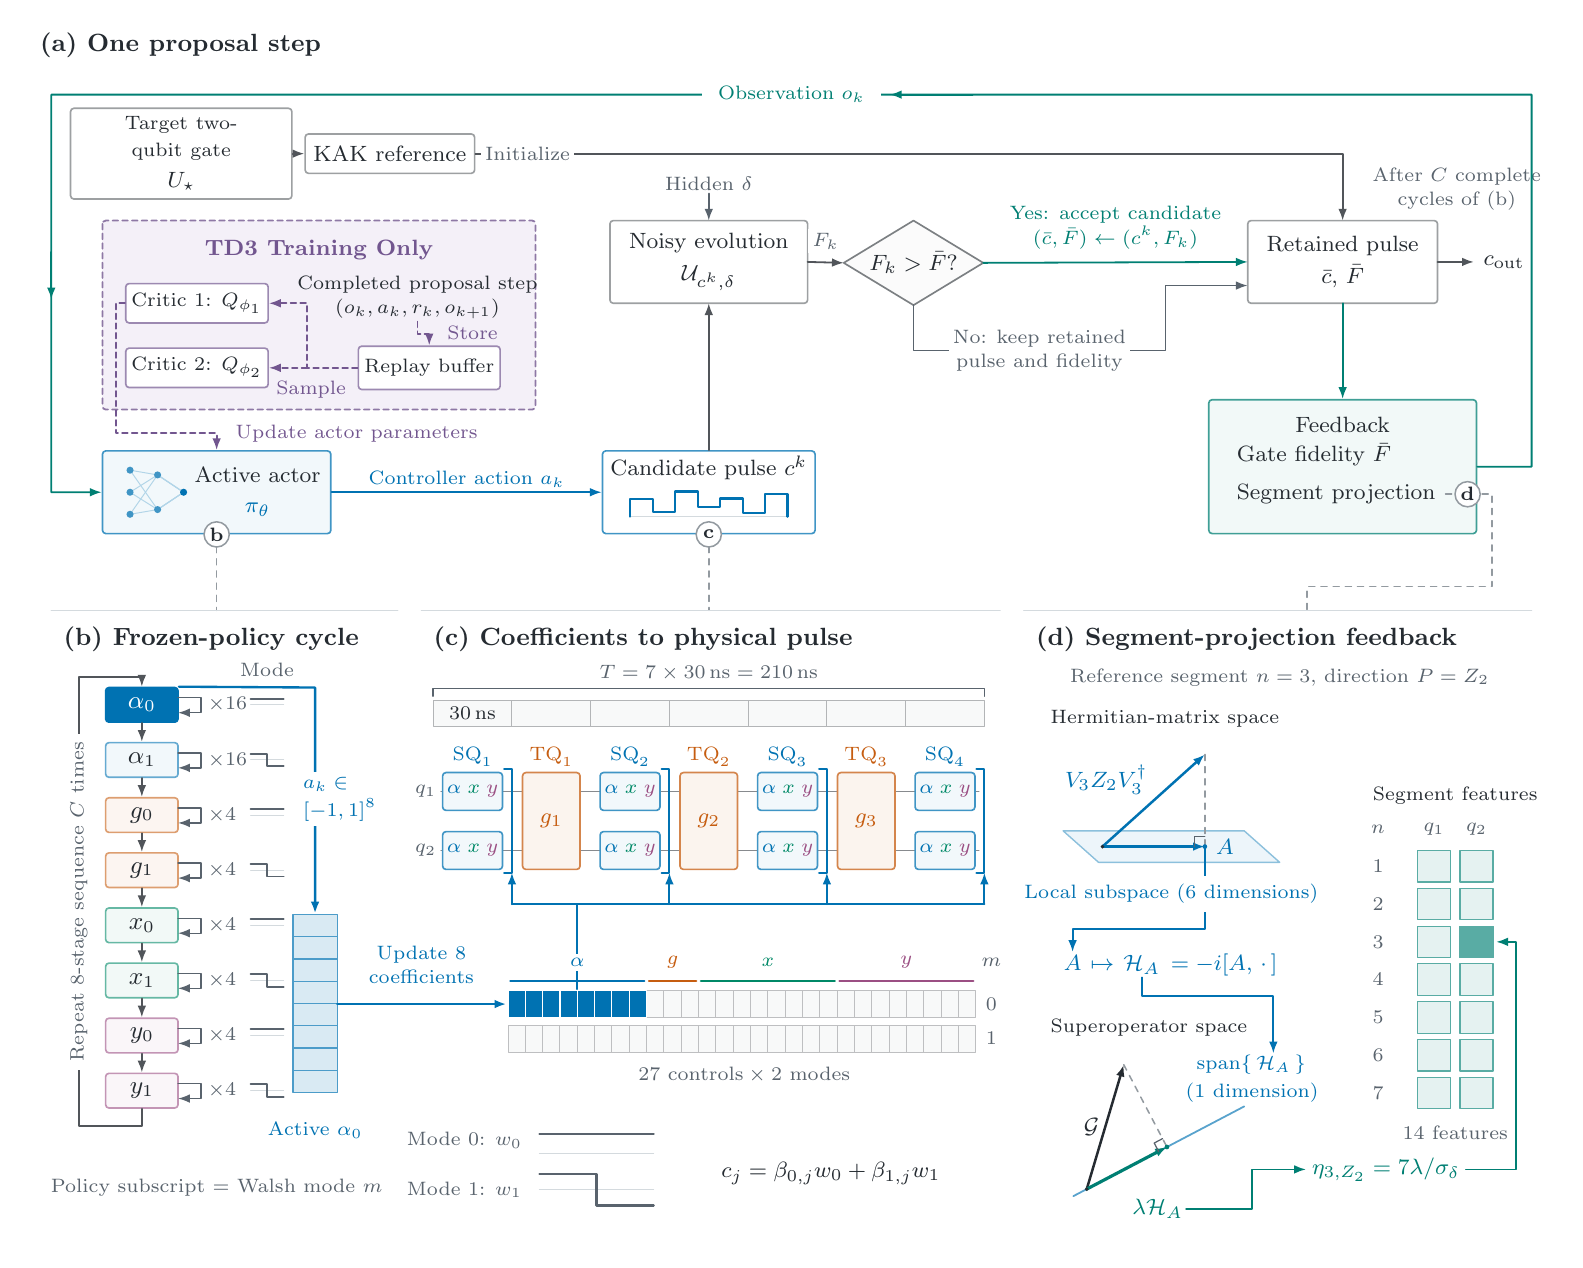
\begin{tikzpicture}[x=1cm,y=-1cm,
    font=\fontsize{8}{9.5}\selectfont,
    text=ink, line cap=round, line join=round]
    \path[use as bounding box] (0,0) rectangle (19.4,15.40);
    \panelheading{0.15}{0.22}{(a) One proposal step}

\node[box,text width=2.6cm,minimum height=0.95cm] (target)
    at (1.95,1.6) {{\fontsize{7.5}{9}\selectfont Target two-qubit gate}\\[2pt]$U_\star$};
\node[box,minimum width=1.75cm,minimum height=0.5cm] (kak)
    at (4.6,1.6) {KAK reference};
\draw[flow] (target.east) -- (kak.west);

\node[box,text width=2.3cm,minimum height=1.05cm,anchor=north,
    outer sep=0pt] (simulator)
    at (8.65,2.45) {Noisy evolution\\[2pt]$\mathcal U_{c^k,\delta}$};
\node[diamond,draw=ink!60,fill=ink!2,line width=0.6pt,
    minimum width=1.7cm,minimum height=1.05cm,inner sep=1pt,
    align=center,aspect=1.65,anchor=north,outer sep=0pt] (acceptance)
    at (11.25,2.45) {$F_k>\bar F$?};
\node[box,text width=2.2cm,minimum height=1.05cm,anchor=north,
    outer sep=0pt] (retained)
    at (16.70,2.45) {Retained pulse\\[2pt]$\bar c,\,\bar F$};
\draw[flow] (kak.east) -- (16.70,1.6) -- (retained.north);
\node[edgelabel] at (6.35,1.6) {Initialize};
\draw[flow] (simulator.east) -- (acceptance.west)
    node[midway,above,edgelabel,yshift=3pt] {$F_k$};
\draw[feedbackflow] (acceptance.east) -- (retained.west)
    node[midway,above,edgelabel,text=feedbackgreen,yshift=3pt]
    {Yes: accept candidate\\$(\bar c,\bar F)\leftarrow(c^k,F_k)$};
\coordinate (keepEntry) at ([yshift=-0.30cm]retained.west);
\draw[flow,draw=muted] (acceptance.south) -- (11.25,4.10)
    -- (14.45,4.10) |- (keepEntry);
\node[edgelabel] at (12.85,4.10)
    {No: keep retained\\pulse and fidelity};

\node[smallnote] (noise) at (8.65,1.98) {Hidden $\delta$};
\draw[flow,draw=muted] (noise.south) -- (simulator.north);
\node[align=center] (output) at ($(retained.center)+(2.05,0)$)
    {$c_{\mathrm{out}}$};
\draw[flow] (retained.east) -- (output.west);
\node[smallnote,align=center] at (18.15,2.05)
    {After $C$ complete\\cycles of (b)};

\begin{scope}[shift={(0,1.25)}]
\node[localbox,minimum width=2.9cm,minimum height=1.05cm] (controller)
    at (2.4,4.65) {};
\foreach \u in {4.37,4.65,4.93}
    \foreach \v in {4.43,4.87}
        \draw[draw=localblue!30,line width=0.35pt]
            (1.3,\u) -- (1.65,\v) -- (1.98,4.65);
\foreach \y in {4.37,4.65,4.93}
    \fill[localblue!75] (1.3,\y) circle[radius=0.045cm];
\foreach \y in {4.43,4.87}
    \fill[localblue!75] (1.65,\y) circle[radius=0.045cm];
\fill[localblue] (1.98,4.65) circle[radius=0.045cm];
\node at (2.92,4.43) {Active actor};
\node[text=localblue] at (2.92,4.87) {$\pi_\theta$};
\end{scope}

% Completed proposal steps supply transitions, including rejected proposals.
\draw[draw=trainingpurple!80,fill=trainingfill,line width=0.65pt,
    rounded corners=1.2pt,dash pattern=on 2pt off 1.5pt]
    (0.95,2.45) rectangle (6.45,4.85);
\node[text=trainingpurple,font=\fontsize{8.5}{10}\selectfont\bfseries]
    at (3.70,2.82) {TD3 Training Only};
\node[smallnote,text=ink] (transition) at (4.95,3.42)
    {Completed proposal step\\$(o_k,a_k,r_k,o_{k+1})$};
\node[box,draw=trainingpurple!70,minimum width=1.80cm,minimum height=0.55cm,
    font=\fontsize{7.3}{8.7}\selectfont,inner sep=2pt]
    (replay) at (5.10,4.32) {Replay buffer};
\node[box,draw=trainingpurple!70,minimum width=1.70cm,minimum height=0.50cm,
    font=\fontsize{7.3}{8.7}\selectfont,inner sep=2pt]
    (criticOne) at (2.15,3.50) {Critic 1: $Q_{\phi_1}$};
\node[box,draw=trainingpurple!70,minimum width=1.70cm,minimum height=0.50cm,
    font=\fontsize{7.3}{8.7}\selectfont,inner sep=2pt]
    (criticTwo) at (2.15,4.32) {Critic 2: $Q_{\phi_2}$};
\draw[flow,draw=trainingpurple,dash pattern=on 2pt off 1.5pt]
    (transition.south) -- (4.95,3.89) -- (5.10,3.89) -- (replay.north);
\node[smallnote,text=trainingpurple] at (5.65,3.88) {Store};
\draw[flow,draw=trainingpurple,dash pattern=on 2pt off 1.5pt]
    (replay.west) -- (3.55,4.32) -- (3.55,3.50) -- (criticOne.east);
\draw[flow,draw=trainingpurple,dash pattern=on 2pt off 1.5pt]
    (3.55,4.32) -- (criticTwo.east);
\node[smallnote,text=trainingpurple] at (3.60,4.60)
    {Sample};
\draw[flow,draw=trainingpurple,dash pattern=on 2pt off 1.5pt]
    (criticOne.west) -- (1.12,3.50) -- (1.12,5.15)
    -- (2.40,5.15) -- (controller.north);
\node[smallnote,text=trainingpurple,anchor=west]
    at (2.60,5.15) {Update actor parameters};

\begin{scope}[shift={(0,1.25)}]
\node[box,draw=localblue!75,minimum width=2.7cm,
    minimum height=1.05cm] (candidate) at (8.65,4.65) {};
\node at (8.65,4.34) {Candidate pulse $c^k$};
\draw[draw=rulegray,line width=0.4pt] (7.65,4.96) -- (9.65,4.96);
\draw[draw=localblue,line width=0.8pt]
    (7.65,4.96) -- (7.65,4.74) -- (7.94,4.74) -- (7.94,4.9)
    -- (8.22,4.9) -- (8.22,4.64) -- (8.51,4.64) -- (8.51,4.84)
    -- (8.79,4.84) -- (8.79,4.73) -- (9.08,4.73) -- (9.08,4.91)
    -- (9.36,4.91) -- (9.36,4.67) -- (9.65,4.67) -- (9.65,4.96);

\node[feedbackbox,minimum width=3.4cm,minimum height=1.70cm,anchor=south]
    (feedback) at ($(controller.south)+(14.30,0)$) {};
\node at ($(feedback.center)+(0,-0.53)$) {Feedback};
\node[anchor=west,text=ink,inner sep=0pt]
    at ($(feedback.center)+(-1.35,-0.15)$)
    {Gate fidelity $\bar F$};
\node[anchor=west,text=ink,inner sep=0pt] (segmentFeedback)
    at ($(feedback.center)+(-1.35,0.35)$) {Segment projection};
\end{scope}

\draw[flow,draw=localblue] (controller.east) -- (candidate.west)
    node[midway,above,edgelabel,text=localblue] {Controller action $a_k$};
\draw[flow] (candidate.north) -- (simulator.south);
\draw[feedbackflow] (retained.south) -- (feedback.north);
\draw[feedbackflow] (feedback.east) -| (19.1,0.85)
    -- (0.3,0.85) -- (0.3,5.90) -- (controller.west);
\draw[feedbackflow] (12.0,0.85) -- (10.95,0.85);
\draw[feedbackflow] (0.3,2.85) -- (0.3,3.45);
\node[edgelabel,text=feedbackgreen,inner xsep=6pt] at (9.7,0.85)
    {Observation $o_k$};

\foreach \name/\x/\letter in {controller/2.4/b,candidate/8.65/c} {
    \draw[detail] (\name.south) -- (\x,7.40);
    \node[tag] at (\name.south) {\letter};
}
\draw[detail] ([xshift=0.12cm]segmentFeedback.east) -| (18.60,7.10)
    -- (16.25,7.10) -- (16.25,7.40);
\node[tag] at ($(segmentFeedback.east)+(0.40,0)$) {d};

    \begin{scope}[shift={(0,1.25)}]
    \draw[separator] (0.3,6.15) -- (4.7,6.15);
\panelheading{0.45}{6.52}{(b) Frozen-policy cycle}

\node[policy,draw=localblue,fill=localblue,text=white] (alpha0)
    at (1.45,7.35) {$\alpha_0$};
\node[policy,draw=localblue!60,fill=localblue!5] (alpha1)
    at (1.45,8.05) {$\alpha_1$};
\node[policy,draw=exchangeorange!60,fill=exchangeorange!6] (g0)
    at (1.45,8.75) {$g_0$};
\node[policy,draw=exchangeorange!60,fill=exchangeorange!6] (g1)
    at (1.45,9.45) {$g_1$};
\node[policy,draw=xgreen!60,fill=xgreen!5] (x0)
    at (1.45,10.15) {$x_0$};
\node[policy,draw=xgreen!60,fill=xgreen!5] (x1)
    at (1.45,10.85) {$x_1$};
\node[policy,draw=ymagenta!60,fill=ymagenta!5] (y0)
    at (1.45,11.55) {$y_0$};
\node[policy,draw=ymagenta!60,fill=ymagenta!5] (y1)
    at (1.45,12.25) {$y_1$};
\foreach \a/\b in {alpha0/alpha1,alpha1/g0,g0/g1,g1/x0,x0/x1,x1/y0,y0/y1}
    \draw[flow] (\a.south) -- (\b.north);
\foreach \y/\steps in {7.35/16,8.05/16,8.75/4,9.45/4,10.15/4,10.85/4,11.55/4,12.25/4} {
    \draw[flow,draw=muted,line width=0.5pt]
        (1.91,{\y-0.09}) -- (2.2,{\y-0.09})
        -- (2.2,{\y+0.10}) -- (1.91,{\y+0.10});
    \node[smallnote,anchor=west,inner xsep=0pt] at (2.28,\y) {$\times\steps$};
}
\node[smallnote] at (3.04,6.9) {Mode};
\foreach \y/\m in {7.35/0,8.05/1,8.75/0,9.45/1,10.15/0,10.85/1,11.55/0,12.25/1} {
    \draw[draw=rulegray,line width=0.35pt] (2.83,\y) -- (3.25,\y);
    \ifnum\m=0
        \draw[draw=muted,line width=0.7pt]
            (2.83,{\y-0.08}) -- (3.25,{\y-0.08});
    \else
        \draw[draw=muted,line width=0.7pt]
            (2.83,{\y-0.08}) -- (3.04,{\y-0.08})
            -- (3.04,{\y+0.08}) -- (3.25,{\y+0.08});
    \fi
}
\draw[flow] (y1.south) -- (1.45,12.70) -- (0.65,12.70)
    -- (0.65,7.0) -- (1.45,7.0) -- (alpha0.north);
\node[smallnote,rotate=90,fill=white,inner xsep=3pt] at (0.65,9.85)
    {Repeat 8-stage sequence $C$ times};

\draw[flow,draw=localblue,line width=0.85pt] (alpha0.north east)
    -- (3.65,7.13) -- (3.65,10.0);
\node[edgelabel,text=localblue,anchor=west,align=left,
    inner xsep=2pt,inner ysep=2pt]
    at (3.42,8.55) {$a_k\in$\\[1pt]$[-1,1]^8$};
\draw[draw=localblue!70,fill=localblue!15,line width=0.45pt]
    (3.37,10.01) rectangle (3.93,12.275);
\foreach \r in {1,...,7} {
    \pgfmathsetmacro{\y}{10.01+\r*2.265/8}
    \draw[draw=localblue!70,line width=0.45pt]
        (3.37,\y) -- (3.93,\y);
}
\node[smallnote,text=localblue] at (3.65,12.75) {Active $\alpha_0$};
\node[smallnote] at (2.4,13.48) {Policy subscript = Walsh mode $m$};

    \draw[separator] (5.0,6.15) -- (12.35,6.15);
\panelheading{5.15}{6.52}{(c) Coefficients to physical pulse}

\node[smallnote] at (8.65,6.94)
    {$T=7\times30\,\mathrm{ns}=210\,\mathrm{ns}$};
\draw[draw=muted,line width=0.5pt]
    (5.15,7.24) -- (5.15,7.14) -- (12.15,7.14) -- (12.15,7.24);
\foreach \j in {0,...,6} {
    \draw[draw=ink!35,fill=ink!3,line width=0.4pt]
        ({5.15+\j},7.30) rectangle ++(1,0.32);
}
\node[smallnote,text=ink] at (5.65,7.46) {$30\,\mathrm{ns}$};

\begin{scope}[yshift=-1.05cm]
\draw[draw=ink!55,line width=0.5pt] (5.25,7.4) -- (12.08,7.4);
\draw[draw=ink!55,line width=0.5pt] (5.25,8.15) -- (12.08,8.15);
\node[smallnote,anchor=east] at (5.23,7.4) {$q_1$};
\node[smallnote,anchor=east] at (5.23,8.15) {$q_2$};
\foreach \x/\r in {5.65/1,7.65/2,9.65/3,11.65/4} {
    \node[smallnote,text=localblue] at (\x,6.96) {$\mathrm{SQ}_{\r}$};
    \foreach \y in {7.4,8.15} {
        \node[localbox,minimum width=0.76cm,minimum height=0.48cm,
            inner sep=1pt,font=\fontsize{7.4}{8.5}\selectfont]
            at (\x,\y) {$\textcolor{localblue}{\alpha}\;\textcolor{xgreen}{x}\;\textcolor{ymagenta}{y}$};
    }
}
\foreach \x/\r in {6.65/1,8.65/2,10.65/3} {
    \node[smallnote,text=exchangeorange] at (\x,6.96) {$\mathrm{TQ}_{\r}$};
    \node[exchangebox,minimum width=0.73cm,minimum height=1.23cm,
        inner sep=1pt,text=exchangeorange] at (\x,7.775) {$g_{\r}$};
}

% One family/mode block spans several physical segments.
\draw[draw=localblue,line width=0.75pt] (6.98,9.91) -- (6.98,8.83);
\draw[draw=localblue,line width=0.75pt] (6.15,8.83) -- (12.15,8.83);
\foreach \x in {5.65,7.65,9.65,11.65} {
    \draw[draw=localblue,line width=0.75pt]
        ({\x+0.40},7.12) -- ({\x+0.50},7.12)
        -- ({\x+0.50},8.43) -- ({\x+0.40},8.43);
    \draw[flow,draw=localblue,line width=0.75pt]
        ({\x+0.50},8.83) -- ({\x+0.50},8.43);
}

\begin{scope}[yshift=-0.35cm]
\foreach \x/\family/\familycolor in
    {6.98/\alpha/localblue,8.19/g/exchangeorange,9.40/x/xgreen,11.16/y/ymagenta}
    \node[smallnote,text=\familycolor,fill=white,inner sep=1.5pt]
        at (\x,9.22) {$\family$};
\foreach \left/\right/\familycolor in
    {6.10/7.86/localblue,7.86/8.52/exchangeorange,8.52/10.28/xgreen,10.28/12.04/ymagenta}
    \draw[draw=\familycolor,line width=0.85pt]
        ({\left+0.03},9.46) -- ({\right-0.03},9.46);
\node[smallnote] at (12.24,9.22) {$m$};
\foreach \m/\y in {0/9.58,1/10.02} {
    \foreach \j in {0,...,26} {
        \pgfmathsetmacro{\x}{6.1+\j*0.22}
        \draw[draw=ink!30,fill=ink!3,line width=0.35pt]
            (\x,\y) rectangle ++(0.22,0.34);
    }
    \node[smallnote] at (12.24,{\y+0.17}) {$\m$};
}
\foreach \j in {0,...,7} {
    \pgfmathsetmacro{\x}{6.1+\j*0.22}
    \draw[draw=white,line width=0.4pt,fill=localblue]
        (\x,9.58) rectangle ++(0.22,0.34);
}
\node[smallnote] at (9.1,10.65) {$27\text{ controls}\times2\text{ modes}$};
\end{scope}

\begin{scope}[yshift=-0.60cm]
\node[smallnote,anchor=east] at (6.32,11.23) {Mode 0: $w_0$};
\node[smallnote,anchor=east] at (6.32,11.86) {Mode 1: $w_1$};
\draw[draw=rulegray,line width=0.4pt] (6.5,11.4) -- (7.95,11.4);
\draw[draw=rulegray,line width=0.4pt] (6.5,11.86) -- (7.95,11.86);
\draw[draw=muted,line width=0.85pt] (6.5,11.15) -- (7.95,11.15);
\draw[draw=muted,line width=0.85pt] (6.5,11.66) -- (7.225,11.66)
    -- (7.225,12.06) -- (7.95,12.06);
\node at (10.2,11.65) {$c_j=\beta_{0,j}w_0+\beta_{1,j}w_1$};
\end{scope}
\end{scope}

    \begin{scope}[shift={(0.8,0)}]
    \draw[separator] (11.85,6.15) -- (18.3,6.15);
\panelheading{12.0}{6.52}{(d) Segment-projection feedback}

\node[smallnote] at (15.10,7.00)
    {Reference segment $n=3$, direction $P=Z_2$};
\node[smallnote,anchor=west,text=ink] at (12.15,7.53)
    {Hermitian-matrix space};

% A plane schematically represents the six-dimensional local subspace.
\filldraw[draw=localblue!45,fill=localblue!7,line width=0.5pt]
    (12.35,8.95) -- (14.65,8.95) -- (15.10,9.35)
    -- (12.80,9.35) -- cycle;
\coordinate (localOrigin) at (12.85,9.15);
\coordinate (localFoot) at (14.15,9.15);
\coordinate (transportedDirection) at (14.15,7.98);
\draw[flow,draw=localblue,line width=0.9pt]
    (localOrigin) -- (transportedDirection);
\node[text=localblue,anchor=south east,inner sep=2pt]
    at ($(localOrigin)!0.5!(transportedDirection)$)
    {$V_3 Z_2 V_3^\dagger$};
\draw[detail] (transportedDirection) -- (localFoot);
\draw[flow,draw=localblue,line width=1.05pt] (localOrigin) -- (localFoot);
\draw[draw=muted,line width=0.45pt]
    (14.02,9.15) -- (14.02,9.02) -- (14.15,9.02);
\fill[ink] (localOrigin) circle[radius=0.025cm];
\fill[localblue] (localFoot) circle[radius=0.03cm];
\node[text=localblue,anchor=west,inner sep=1pt]
    at (14.25,9.15) {$A$};
% The commutator map connects the two spaces, without another projection.
\node[text=localblue,inner sep=1pt] (commutatorGenerator)
    at (13.35,10.65) {$\mathcal H_A$};
\node[text=localblue,anchor=base east,inner sep=1pt] (commutatorInput)
    at ([xshift=-0.45cm]commutatorGenerator.base west) {$A$};
\node[text=localblue,anchor=base,inner sep=0pt]
    at ($(commutatorInput.base east)!0.5!(commutatorGenerator.base west)$)
    {$\mapsto$};
\node[text=localblue,anchor=base west,inner sep=0pt]
    at ([xshift=1pt]commutatorGenerator.base east) {$\,=-i[A,\,\cdot\,]$};
\draw[flow,draw=localblue] (localFoot) -- (14.15,10.20)
    -| (commutatorInput.north);
\node[smallnote,text=localblue,fill=white,inner sep=3pt]
    at (13.725,9.75) {Local subspace (6 dimensions)};

\begin{scope}[shift={(0,0.80)}]
\node[smallnote,anchor=west,text=ink] at (12.15,10.65)
    {Superoperator space};

% A short line depicts the one-dimensional real span of the superoperator.
\coordinate (projectionOrigin) at (12.65,12.70);
\coordinate (projectionResidual) at (13.12,11.12);
\coordinate (projectionDirection) at (14.65,11.65);
\coordinate (projectionFoot) at
    ($(projectionOrigin)!(projectionResidual)!(projectionDirection)$);
\draw[draw=localblue!65,line width=0.65pt]
    (12.48,12.7893) -- (projectionDirection);
\node[smallnote,text=localblue,inner sep=1pt] (spanGenerator)
    at (15.02,11.12) {$\mathcal H_A$};
\node[smallnote,text=localblue,anchor=base east,inner sep=0pt]
    at (spanGenerator.base west) {$\operatorname{span}\{$};
\node[smallnote,text=localblue,anchor=base west,inner sep=0pt]
    at (spanGenerator.base east) {$\}$};
\node[smallnote,text=localblue] at (14.75,11.48) {(1 dimension)};
\draw[flow,draw=ink,line width=0.9pt]
    (projectionOrigin) -- (projectionResidual);
\node[anchor=east,inner sep=2pt]
    at ($(projectionOrigin)!0.5!(projectionResidual)$)
    {$\mathcal G$};
\draw[detail] (projectionResidual) -- (projectionFoot);
\draw[feedbackflow,line width=1.15pt]
    (projectionOrigin) -- (projectionFoot);
\fill[ink] (projectionOrigin) circle[radius=0.025cm];
\fill[feedbackgreen] (projectionFoot) circle[radius=0.03cm];
\coordinate (projectionAlong) at
    ($(projectionFoot)!0.12cm!(projectionOrigin)$);
\coordinate (projectionNormal) at
    ($(projectionFoot)!0.12cm!(projectionResidual)$);
\draw[draw=muted,line width=0.45pt]
    (projectionAlong) --
    ($(projectionAlong)+(projectionNormal)-(projectionFoot)$) --
    (projectionNormal);
\node[text=feedbackgreen,inner sep=1pt] (projectedMatrix)
    at (13.55,12.95) {$\lambda\mathcal H_A$};
\node[text=feedbackgreen,inner sep=2pt] (segmentFeature)
    at (16.45,12.45) {$\eta_{3,Z_2}=7\lambda/\sigma_\delta$};
\draw[feedbackflow] (projectedMatrix.east) -- (14.75,12.95)
    -- (14.75,12.45) -- (segmentFeature.west);

% Seven rows identify segments; two columns identify qubits.
\node[smallnote,text=ink] at (17.33,7.70) {Segment features};
\node[smallnote] at (16.35,8.13) {$n$};
\node[smallnote] at (17.06,8.13) {$q_1$};
\node[smallnote] at (17.60,8.13) {$q_2$};
\foreach \r in {0,...,6} {
    \pgfmathsetmacro{\y}{8.40+0.48*\r}
    \node[smallnote] at (16.35,{\y+0.20})
        {$\the\numexpr\r+1\relax$};
    \foreach \c in {0,1} {
        \pgfmathsetmacro{\x}{16.85+0.54*\c}
        \draw[draw=feedbackgreen!65,fill=feedbackgreen!10,line width=0.4pt]
            (\x,\y) rectangle ++(0.42,0.40);
    }
}
\draw[draw=feedbackgreen!65,fill=feedbackgreen!65,line width=0.4pt]
    (17.39,9.36) rectangle ++(0.42,0.40);
\node[smallnote] at (17.33,11.98) {$14$ features};
\draw[feedbackflow] (segmentFeature.east) -- (18.10,12.45)
    -- (18.10,9.56) -- (17.85,9.56);
\end{scope}
\draw[flow,draw=localblue] (commutatorGenerator.south) -- (13.35,11.05)
    -| (spanGenerator.north);

    \end{scope}
    \draw[flow,draw=localblue,line width=0.85pt]
        (3.93,11.15) -- (6.08,11.15);
    \node[edgelabel,text=localblue] at (5.0,10.65) {Update 8\\coefficients};
    \end{scope}
\end{tikzpicture}
\end{document}
